\documentclass[a4paper]{scrreprt}
\usepackage{scrextend}
\usepackage[german]{babel}
\usepackage[utf8]{inputenc}
\usepackage[T1]{fontenc}
\usepackage{ae}
\usepackage[bookmarks,bookmarksnumbered]{hyperref}

%graphics
\usepackage{graphicx}
\graphicspath{ 
  {images/high-level/}
  } 
\usepackage[printonlyused]{acronym}
\usepackage{hyperref}
\usepackage{float}

\begin{document}

\title{Entwurf}
\author{Überdurchschnittliche Gruppe}
\maketitle 
\chapter{Übersicht}
\section{Einleitung}
Dieses Dokument beschreibt den Entwurf des Softwaresystemes welches in unserem Pflichtenheft beschrieben wurde. Es verwendet eine objektorientierte Architektur nach dem Model-View-Controller Prinzip. Zusammengehörige Funktionalität wird in Klassen gekapselt. Module sollen leicht austauschbar sein und klar definierte Schnittstellen bieten. Der Entwurf strebt an, modular und damit leicht veränder- und erweiterbar zu sein.

\subsection{abstrakteste Sichtweise}
Die allgemeinste Sicht auf unser Softwaresystem ist Folgende: Wir benötigen
\begin{itemize}
\item Eine "'Quelle"' für eine Beschreibung eines Wahlverfahrens
\item Eine "'Quelle"' für eine Beschreibung der formalen Eigenschaften, welche diese Wahlverfahren erfüllen soll		
\item Eine Überprüfungsinstanz welche Wahlverfahren und Eigenschaften entgegennimmt das Ergebnis der Überprüfung zurückgibt
\item Eine Komponente welche diese Ergebnisse darstellen kann
\item Ein Koordinator, welcher die Koordination zwischen obigen Komponenten übernimmt
\end{itemize}

\begin{figure}[H]
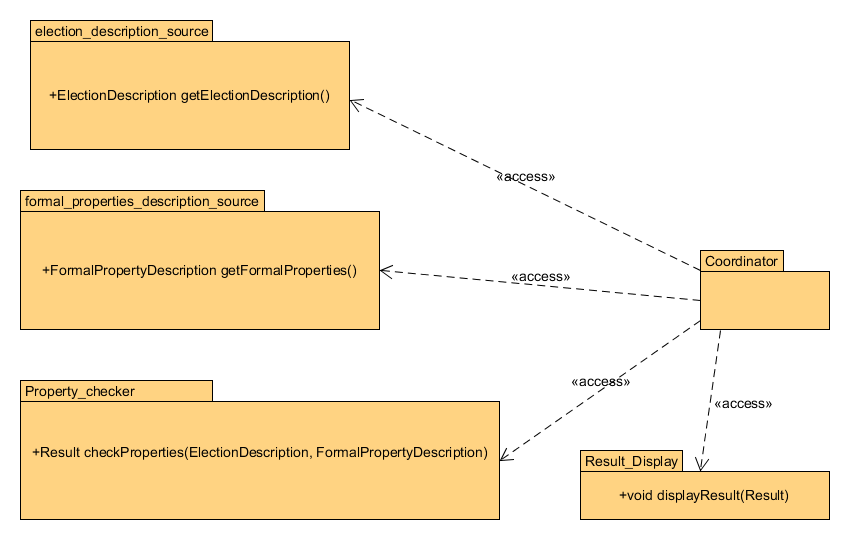
\includegraphics[scale=0.5]{highest-level-general-view.png}
\caption{allgemeinste Sicht auf die Architektur von BEAST}
\label{most_general_view_of_beast_architecture}
\end{figure}

\subsection{Konkrete Sichtweise}
Der Vorteil der abstrakten Beschreibung ist, dass sie quasi unbegrenzte Möglichkeiten liefert und es sehr klar macht, an welchen Stellen man das Programm fundamental ändern kann. Wir werden die Beschreibung des Wahlverfahrens als C-Code implementieren, und die Quelle dafür als C-Editor. Es ist jedoch denkbar, dies in Zukunft durch einen graphischen Editor zu ersetzen, welcher zum Beispiel Flowcharts verwendet. Die formalen Eigenschaften wird in der im Pflichtenheft beschriebenen Syntax gegeben. Als Quelle dient die Eigenschaftenliste welche wiederum den Eigenschafteneditor verwendet. Die Koordination wird von dem Parametereditor übernommen. Zur Überprüfung wird ein bounded model checker verwendet, in unserem Fall speziell der C bounded model checker. Darstellen der Ergebnisse geschieht in der Eigenschaftenliste.  

\begin{figure}[H]
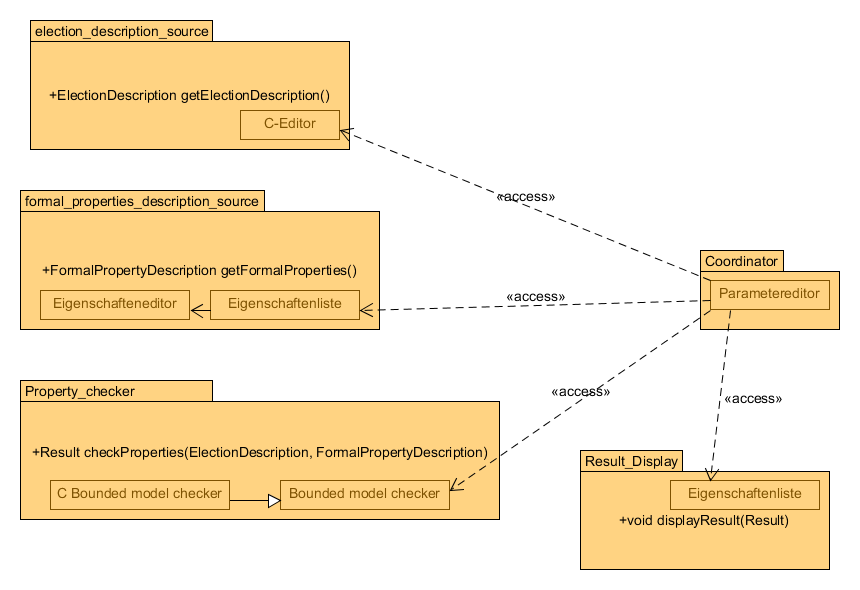
\includegraphics[scale=0.5]{highest-level-concrete-view.png}
\caption{Konkrete Sicht auf die Architektur von BEAST}
\label{concrete_view_of_beast_architecture}
\end{figure}

\section{Überblick über einzelne Komponenten}
Wie bereits erwähnt verwendet der Entwurf eine Einteilung der Komponenten nach dem Model-View-Controller Schema. Dadurch wird unter anderem zwischen interner und externer Darstellung der Daten unterschieden. 

\chapter{Überprüfung der Modelle}

\end{document}